\begin{frame}{Liegt es an der Zusammensetzung der Erdatmosphäre, dass nicht alle Frequenzen durchgelassen werden? Und wie kommt es, dass bestimmte Frequenzbereiche nicht durchgelassen werden?}
  \begin{figure}
    \centering
    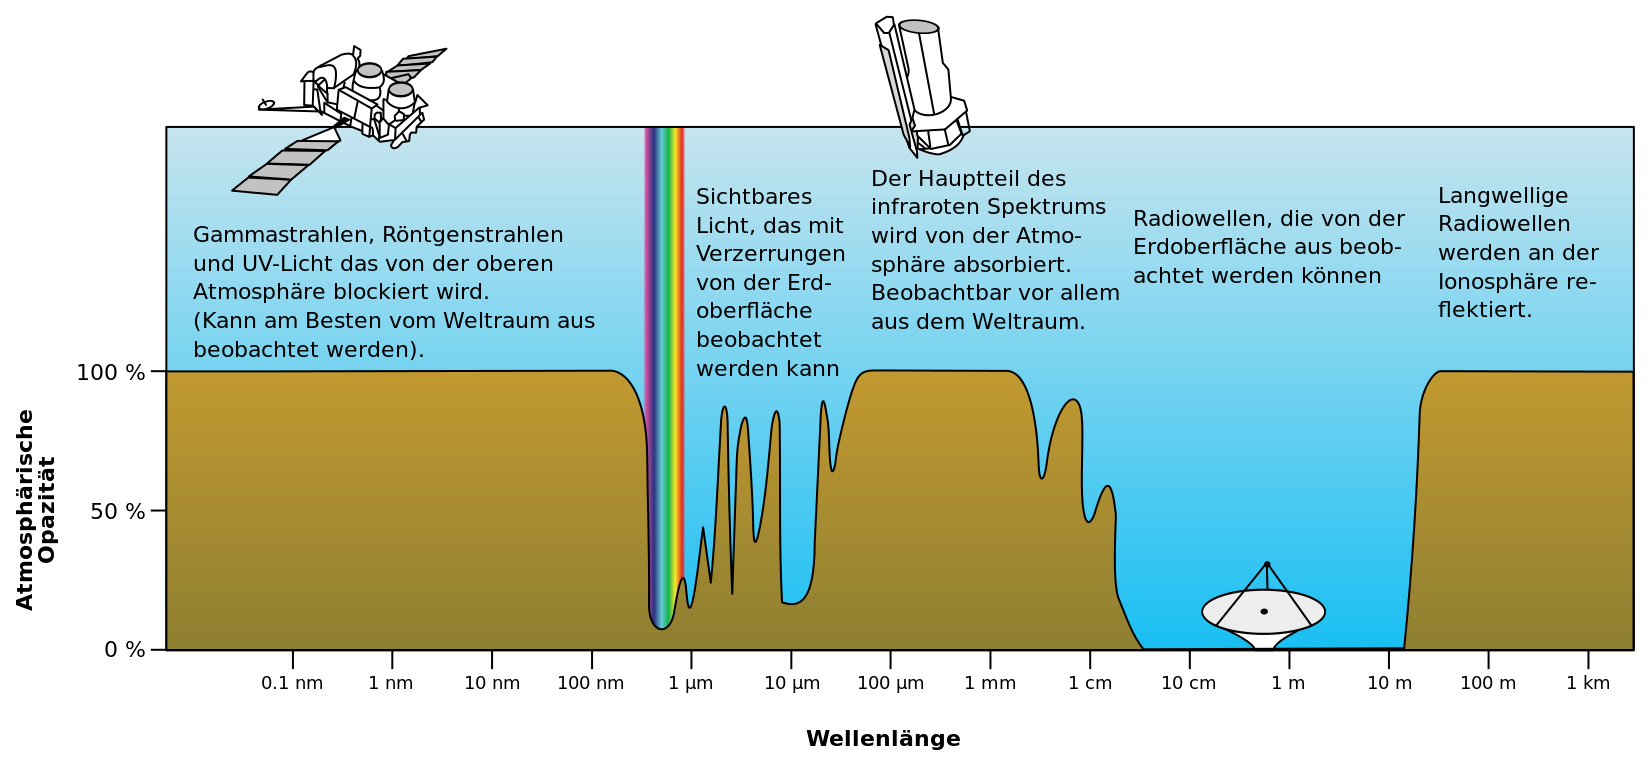
\includegraphics[width=0.9\textwidth]{images/Atmospheric.png}
  \end{figure}
\end{frame}
  \begin{frame}{Liegt es an der Zusammensetzung der Erdatmosphäre, dass nicht alle Frequenzen durchgelassen werden? Und wie kommt es, dass bestimmte Frequenzbereiche nicht durchgelassen werden?}
    \begin{columns}
   \begin{column}{0.4\textwidth}
    \begin{itemize}
        \setlength\itemsep{2em}
      \item Ja es liegt an der Zusammensetzung der Atmosphäre
      \item Gase aborbieren bestimmte Wellenlängen
    \end{itemize}
  \vspace{2em}
  \end{column}
  \begin{column}{0.6\textwidth}
    \begin{figure}
      \centering
      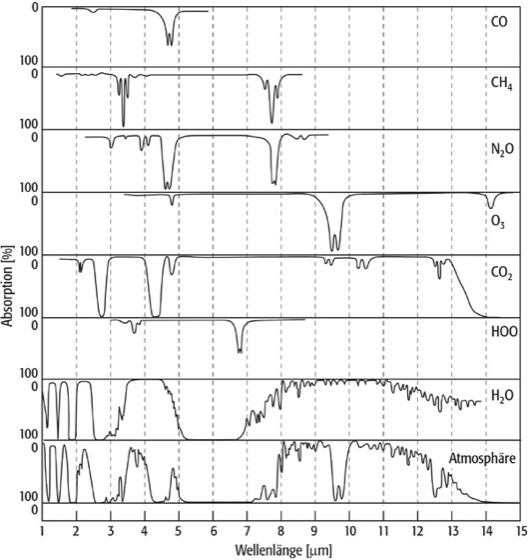
\includegraphics[width=0.65\textwidth]{images/atmo_fen_w.jpg}
    \end{figure}
  \end{column}
    \end{columns}
  \end{frame}


\begin{frame}{}
  \textbf{Warum haben die Sonne / die Sterne ein Schwarzkörperspektrum?}
  \begin{itemize}
    \item Schwarzer Strahler: reflektiert kein Licht, sendet Wärmestrahlung aus die nur von der Oberfläche und Temperatur abhänig ist
    \item Sonne ist auch ein Wärmestrahler
  \end{itemize}
  \vspace{1em}
  \textbf{Was sind Feld-Quanten?}
  \begin{itemize}
    \item Eichbosonen / Austauschteilchen
    \item Photonen, Gluonen, $Z^0$, $W^\pm$
  \end{itemize}
  \vspace{1em}
  \textbf{Wofür ist die Friedmann-Gleichung}
  \begin{itemize}
    \item Beschreibung der Entwicklung des Universums
    \end{itemize}
    \vspace{1em}
    \textbf{Wodurch und wie entstehen Gamma Ray Bursts?}
    \begin{itemize}
      \item  Man weiß es nicht
      \item  Supernova, Neutronenstarmerger
    \end{itemize}
\end{frame}

\begin{frame}{Wodurch genau ist die Rotverschiebung charakterisiert?}
  \begin{columns}
 \begin{column}{0.5\textwidth}
  \begin{itemize}
      \setlength\itemsep{2em}
    \item Kosmische Rotverschiebung aufgrund der Ausdehnung des Universums
    \item Rotverschiebung aufgrund des Dopplereffektes: Bewegung, z.B. bei Spiralgalaxien
  \end{itemize}
  \end{column}
\begin{column}{0.5\textwidth}
  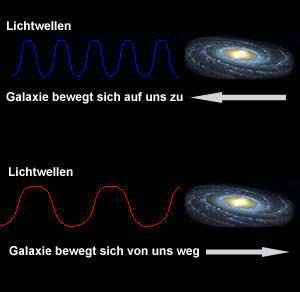
\includegraphics[width=\textwidth]{images/doppler.jpg}
\end{column}
  \end{columns}
\end{frame}

\begin{frame}{Was genau ist das Hubbelgesetz und die Hubbelkonstante und wofür ist es?}
  \begin{columns}
    \begin{column}{0.5\textwidth}
      \begin{itemize}
          \setlength\itemsep{2em}
        \item Hubble Parameter beschreibt die Expansionsrate des Universums:
        \begin{equation*}
          H(t)=\frac{\dot a(t)}{a(t)}
      \end{equation*}
      $a(t)$: Skalenfaktor
      \item $H(t_0)=70\,\frac{\text{km}}{\text{s}\cdot \text{Mpc}}$
      \item Hubble-Gesetz:
      \begin{equation*}
        v=H\cdot r
      \end{equation*}
      \end{itemize}
    \end{column}
    \begin{column}{0.5\textwidth}
  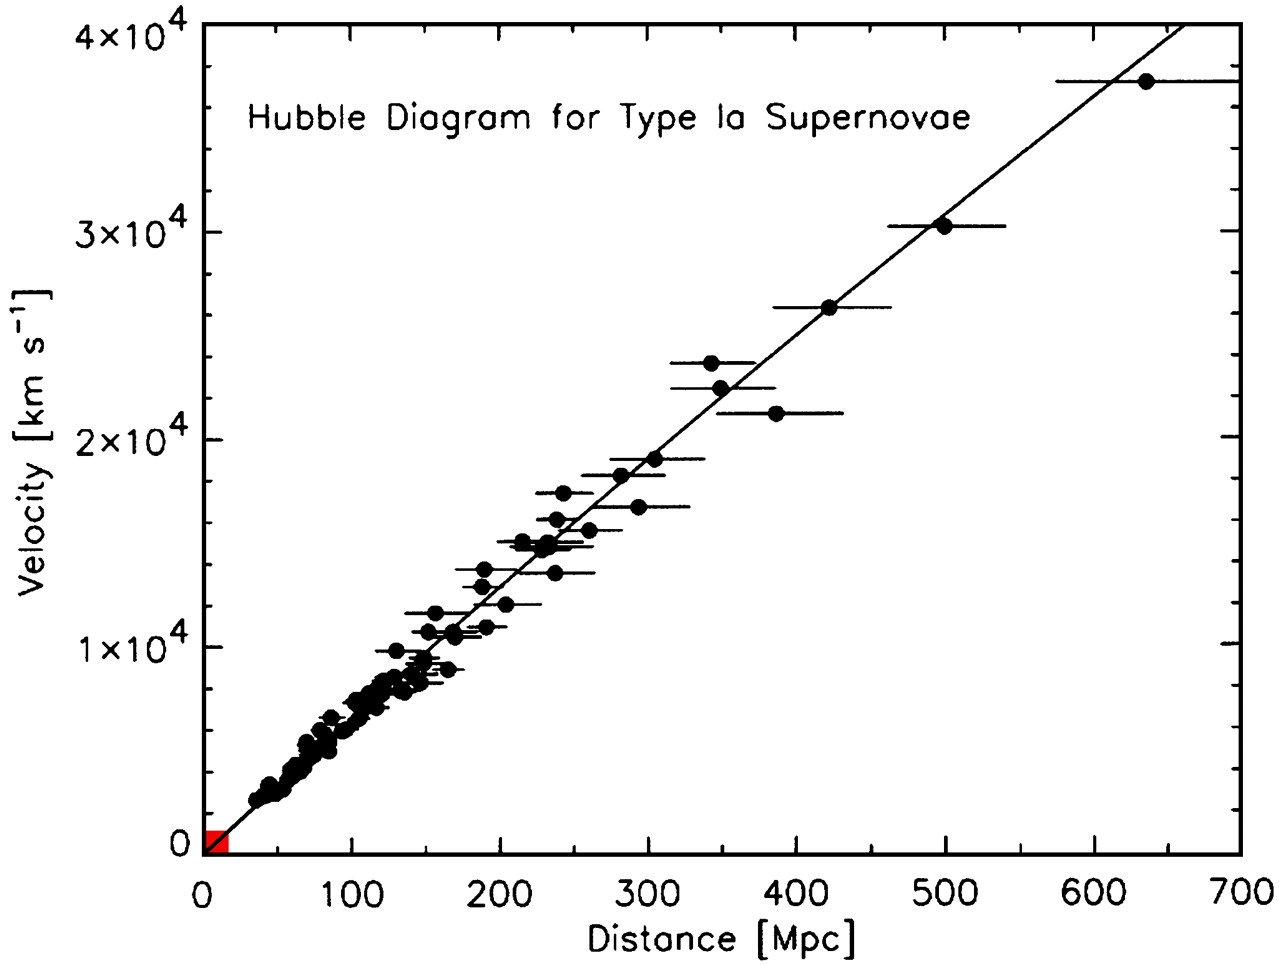
\includegraphics[width=\textwidth]{images/hubble.jpg}
    \end{column}
  \end{columns}
\end{frame}

\begin{frame}{Was genau ist das Wasserstoffbrennen und wodurch entsteht es?}
  \begin{columns}
    \begin{column}{0.5\textwidth}
\begin{itemize}  \setlength\itemsep{2em}
  \item Kernfusion von Wasserstoff zu Helium
  \item Hohe Temperatur (ca $15\cdot10^6\,\text{K}$) und hoher Druck sind Vorausetzung\\
  $\rightarrow$ Gravitationspotential des Sterns
\end{itemize}
    \end{column}
    \begin{column}{0.5\textwidth}
  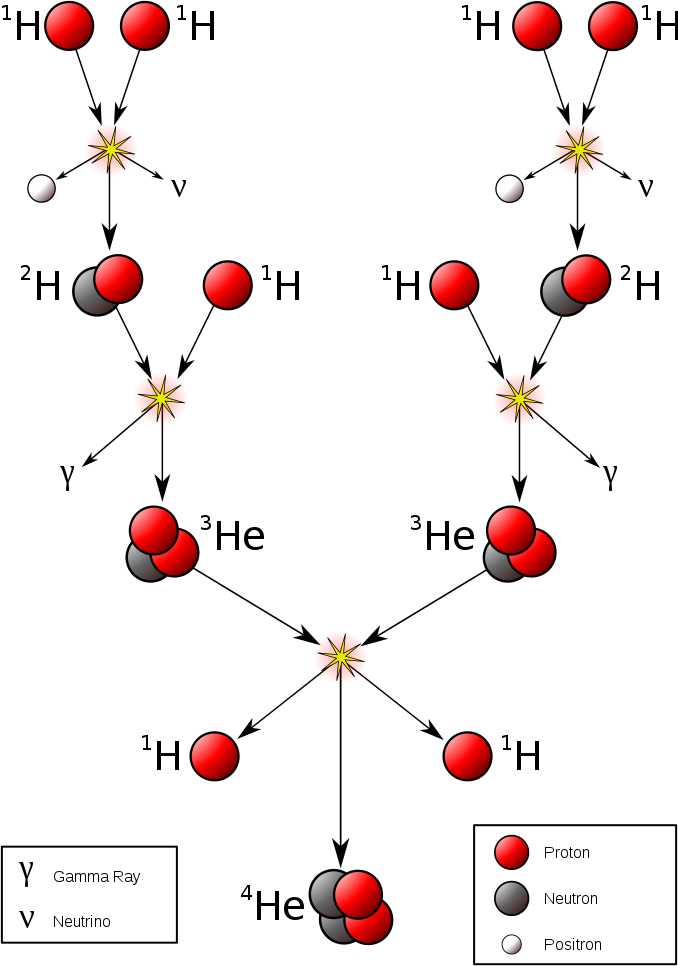
\includegraphics[width=0.65\textwidth]{images/wasserstoff.png}
    \end{column}
  \end{columns}
\end{frame}

\begin{frame}{ }
  \begin{columns}
    \begin{column}[t]{0.5\textwidth}
      \textbf{Wie genau funktioniert der Energietransport bei Sternen?}
\begin{itemize}
  \item Strahlungstransport
  \item Konvektion
  \item Wärmeleitung
  \item Neutrinos
  $\rightarrow$ Gravitationspotential des Sterns
\end{itemize}
\vspace{1em}
\textbf{ Was genau ist das Eddington-Limit?}
\begin{itemize}
  \item Natürliche Begrenzung der Leuchtkraft
  \item Bei Überschreitung des Limits: kein Hydrostatisches Gleichgewicht mehr: Strahlungsdruck dominiert, Stern explodiert
\end{itemize}
\vspace{1em}
\textbf{Wie sieht der Lebeneslauf eines Sternes aus?}
\begin{itemize}
  \item Abhängigkeit von Masse
  \item Vorlesungsfolien!
\end{itemize}
    \end{column}
    \begin{column}[t]{0.5\textwidth}
      \textbf{Aus welchen Elementen bestehen die meisten Sterne?}
      \begin{itemize}
        \item Wasserstoff, Helium
        \item Alte Sterne: Zwiebelschalenmodell
      \end{itemize}
      \vspace{1em}
      \textbf{Warum leben leichte Sterne länger als schwere?}
      \begin{itemize}
        \item 2 $\times$ heller $\rightarrow$ 10 $\times$ mehr Energieabgabe
        \item Wasserstoff ist schneller aufgebraucht
      \end{itemize}
      \vspace{1em}
      \textbf{Was sind typische Ursachen für Dichtefluktuationen, die zur Entstehung neuer Sterne führt?}
      \begin{itemize}
        \item HII Region: große, kalte Molekülwolke
        \item Rotation der Galaxie: Dehimpuls
        \item Wolke fragmentiert: mehere Teilwolken
        \item Enstehung mehrerer Sterne
      \end{itemize}
      \end{column}
  \end{columns}
\end{frame}


\begin{frame}{Worin liegt genau der Unterschied zwischen einer Supernovae Typ I und Supernovae Typ II?}
\begin{columns}
  \begin{column}{0.5\textwidth}
    \textbf{Supernova Typ I}
    \begin{itemize}
      \item Keine Wasserstofflinien
      \item Akkretion der Masse eines Roten Riesens auf einen weißen Stern
      \end{itemize}
      \vspace{1em}
      \textbf{Supernova Typ II}
      \begin{itemize}
        \item Wasserstofflinien, Stern besaß noch Wasserstoffhülle
      \end{itemize}
  \end{column}
  \begin{column}{0.5\textwidth}
      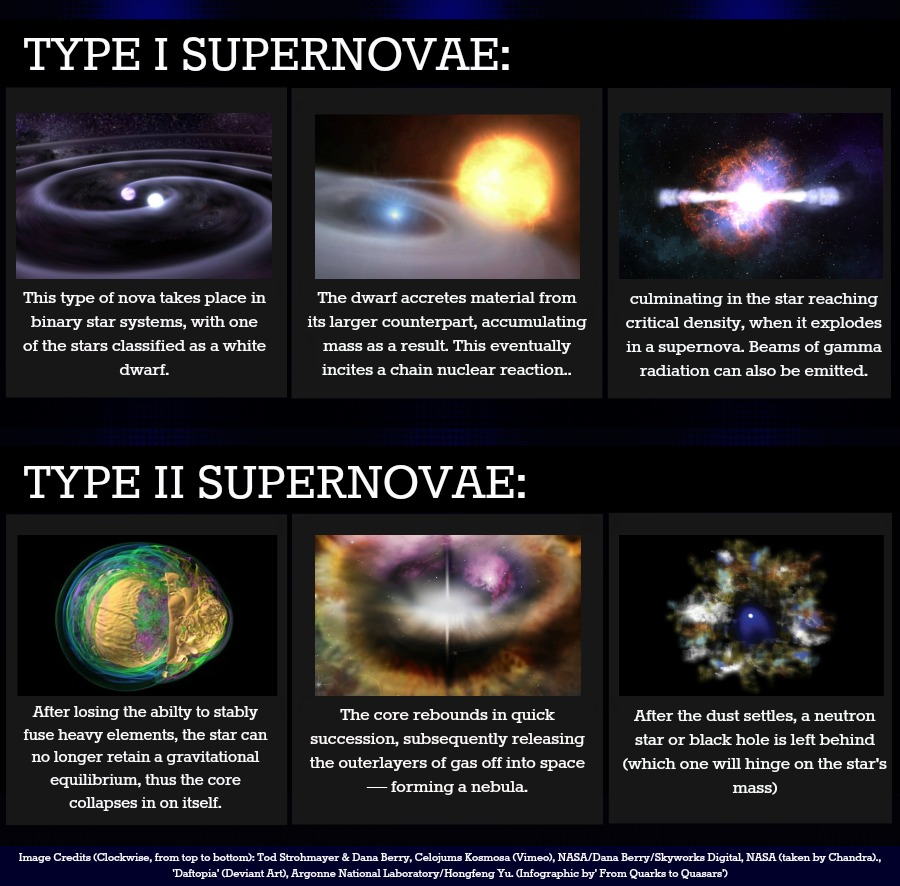
\includegraphics[width=\textwidth]{images/supernova.png}
    \end{column}
\end{columns}
\end{frame}


\begin{frame}{Was genau ist eine Wind-Supernovae und warum hat sie einen anderen Fluss als die SN-ISM? Wofür steht ISM?}
\end{frame}

\begin{frame}{Wie kommt es zur variablen Helligkeit der Cepheiden?}
  \begin{columns}
    \begin{column}{0.5\textwidth}
      \textbf{Kappa-Mechanismus}
\begin{itemize}
  \item Auslöser: Störung verursacht Komprimierung der Materie im Stern in einer Schicht
  \item In der Schicht: Anstieg der Temperatur und des Drucks
  \item Opazität steigt: Strahlung kann nicht nach außen weitergeleitet werden
  \item Äußere Schichten fallen nach innen (fehlender Strahlungsdruck)
  \item Temperaturerhöhung in der Schicht: Expansion $\rightarrow$ Opazität nimmt ab
  \item Strahlung wird abgegeben: Expansion der äußeren Schicht
  \item Freigelassene Energie führt zur Kompression
\end{itemize}
    \end{column}
    \begin{column}{0.5\textwidth}
        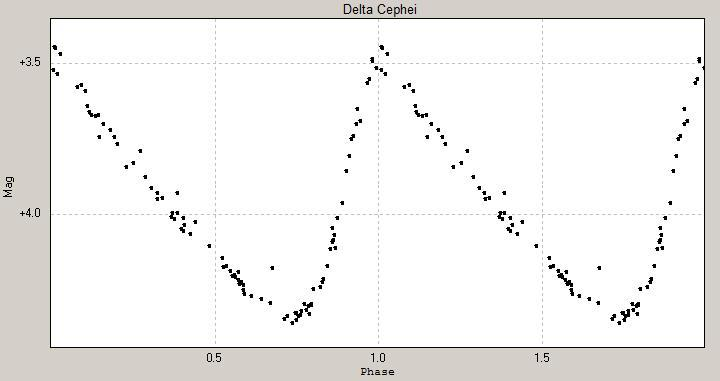
\includegraphics[width=\textwidth]{images/Delta_Cephei.jpg}
      \end{column}
  \end{columns}
\end{frame}
